\section{\neupims Architecture}
\label{sec:architecture}

       
%
\subsection{PIM Microarchitecture for Concurrent Execution}


\niparagraph{Single row buffer for PIM-based accelerator.}
%
Figure~\ref{fig:newton-vs-neupims}(a) depicts the high-level architecture of PIM-based GEMV accelerators that utilize banks equipped with a single row buffer.
%
For a GEMV, the vector operand is first located in the global buffer shared across all banks in a channel.
%
On the contrary, the rows of matrix operand are read from multiple banks simultaneously, exploiting bank-level parallelism, and located at their corresponding row buffers.
%
When the operands are ready, the parallel multipliers and adder tree perform a partial dot-product by reading the broadcast vector input from the global buffer and per-bank row buffers.
%

\niparagraph{Limitation of current PIM-based GEMV accelerators.}
%
Current PIM accelerators~\cite{newton, hbm_pim, aespa} operate in a ``blocked'' mode, preventing the simultaneous executions of NPU\footnote{
%
Henceforth in this paper, ``NPU'' refers exclusively to the device integrated within \neupims, setting it apart from any standalone NPUs.
%
} and PIM. 
%
This limitation arises primarily because the memory bank utilizes a single row buffer that serves two purposes: read/write memory operations and PIM acceleration specifically for GEMV.
%
These modes are managed sequentially, making it impossible to perform simultaneous executions. 
%
While this constraint does not significantly impact PIM system's performance for sole execution of GEMV, it becomes pertinent for LLM inferencing that requires both GEMM and GEMV operations.
%
Addressing this issue, our work aims to facilitate the parallel execution of both modes within the PIM framework. 
%
This advancement is expected to significantly enhance performance in LLM inferencing applications, unlocking the full potential of PIM beyond its current limitations.


\niparagraph{Extending PIM with dual row buffers.}
%
Figure~\ref{fig:newton-vs-neupims}(b) delineates the microarchitecture of \neupims bank. 
%
The memory banks of \neupims are equipped with \emph{dual row buffers}, namely MEM row buffer and PIM row buffer, which are associated with two independent data paths. 
%
Memory (MEM) row buffer is exclusively used for regular memory read/write accesses, whereas PIM row buffer is employed for GEMV operation. 
%
In designing \neupims, our design principle is to minimize the microarchitectural modification since the complication would impose significant area and power costs, lowering the practicality in the real-world system. 
%
Instead, we delegate the complications to the command interface and memory control mechanism, which will be elaborated below.
%

For prototyping and evaluating \neupims, we choose an industry-developed PIM accelerator designed for GEMV, Newton~\cite{newton}.
%
However, note that the proposed techniques in this work are not bounded to the Newton architecture, rather applicable to any GEMV accelerator that follows the standard DRAM microarchitecture and command interface. 

\begin{figure}[t]
        \centering
        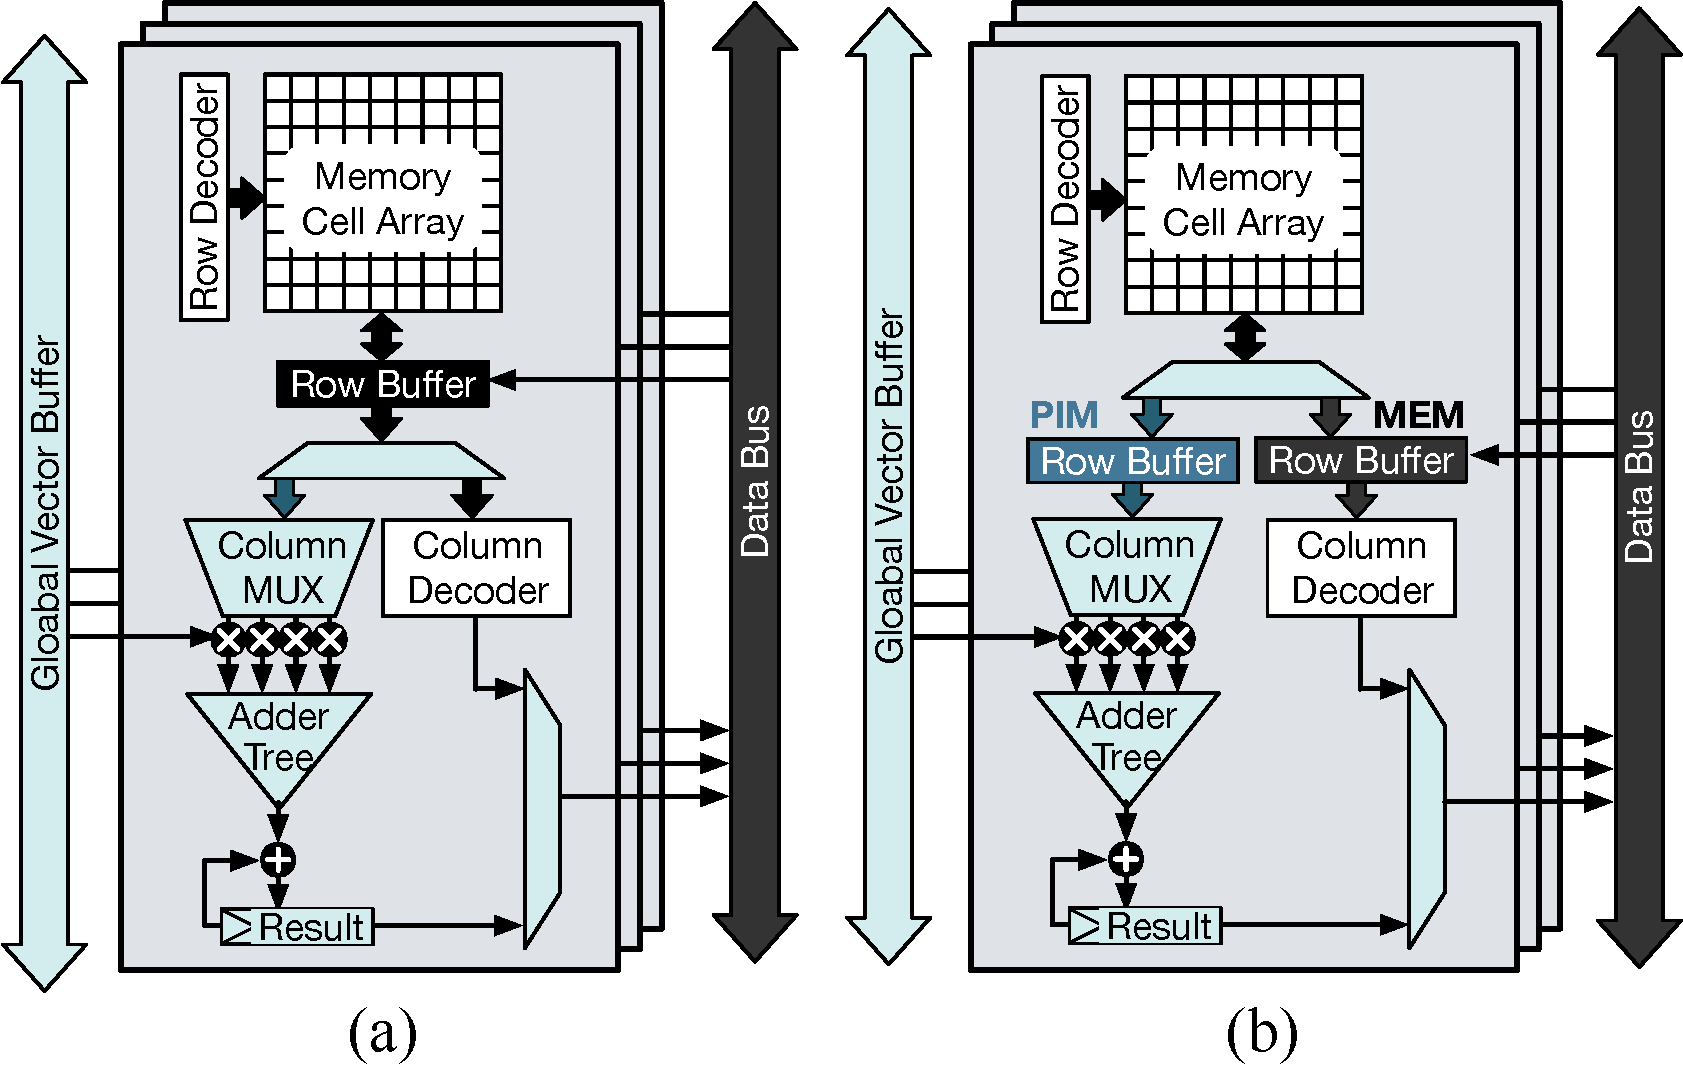
\includegraphics[width=1.0\linewidth]{figure/pim-microarchi.pdf}
        \vspace{-4ex}
        \caption{Microarchitecture of memory banks in (a) existing PIM accelerators with single row buffer banks, and (b) the proposed \neupims with dual row buffer banks.}
        \vspace{-2ex}
        \label{fig:newton-vs-neupims}
\end{figure}

%
\subsection{Memory Command Interface} 
%
%
\niparagraph{Existing command interface for PIM-based GEMV.}
%
We develop the \neupims device using a PIM accelerator with a modified command interface on top of the existing DRAM standard interface.
%
There are four commands that collaboratively operate the PIM.
%
First, to process GEMV in PIM banks, \neupims must copy the operand vector to a global vector buffer shared by the banks within a channel. 
%
\neupims perform this operation using the PIM\_GWRITE command, which copies a specific row of a particular bank to the global vector buffer.
%
Similarly, it needs another command to activate the rows of the operand matrix into PIM row buffers across the banks.
%
For this, the host produces grouped activation commands, called ``PIM\_ACTIVATION'', which activate PIM row buffers of multiple banks simultaneously, usually for 4 banks at a time due to the power constraints (i.e., tFAW).
%
Once all the banks are activated, the host sends ``PIM\_DOTPRODUCT'' command  that performs parallelized dot-product computation, extracting massively larger in-memory bandwidth than host-memory bandwidth. 
%
Finally, the ``PIM\_RDRESULT'' command transfers the accumulated results to the host, ending a round of GEMV operation in PIM. 
%

\begin{figure}[t]
        \centering
        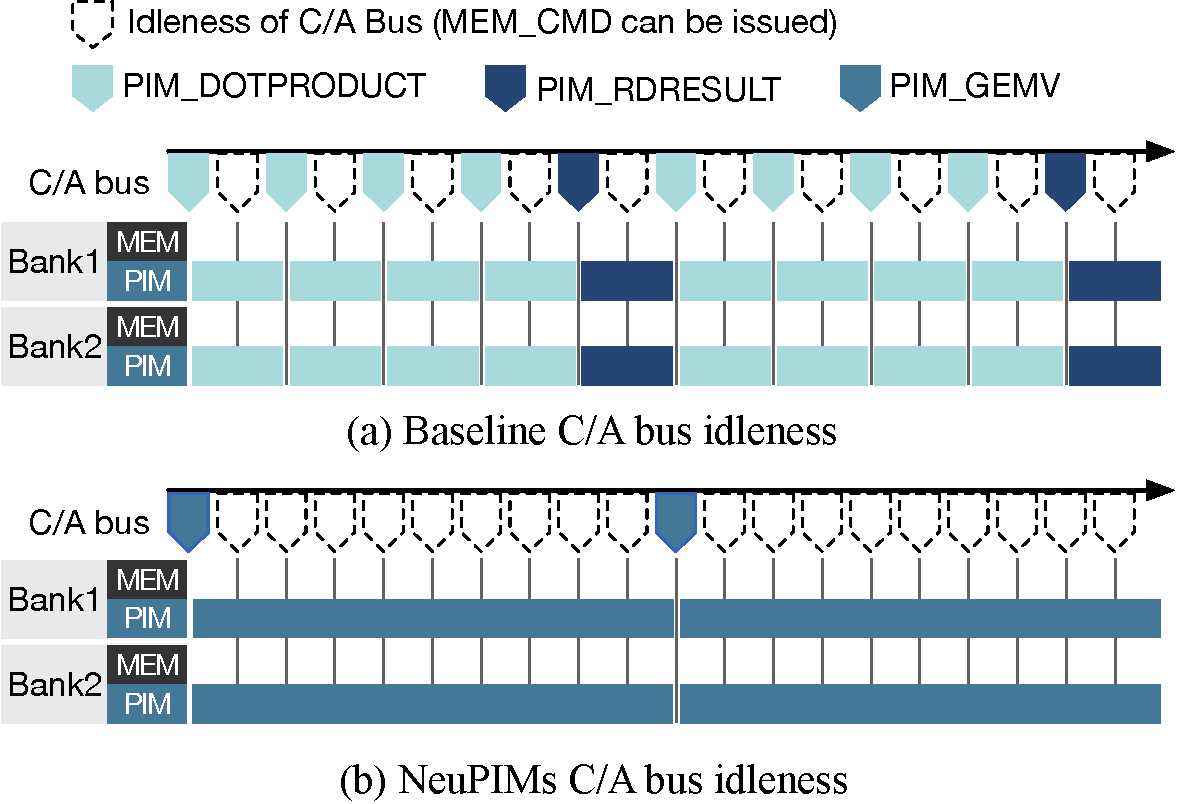
\includegraphics[width=0.9\linewidth]{figure/fig9-command-timing.pdf}
        \vspace{-2ex}
        \caption{PIM command timing comparison.}
        \vspace{-2ex}
        \label{fig:body-pim-cmd-timing}
\end{figure}

\niparagraph{\neupims command interface.}
%
We modify the command interface of baseline PIM by augmenting three additional commands that support new capabilities for \neupims.
%
\begin{table}
\centering
\small % Used small font due to width
\renewcommand{\arraystretch}{1.05}
\caption{List of \neupims commands.}
\footnotesize
\label{tab:neupims-commands}
\vspace{-2ex}
\begin{tabular}{c|c}

\hline
\textbf{Command} & \textbf{Description}                                                                                                                 \\ 
\hline
% GWRITE         & MEM                                                                      & \begin{tabular}[c]{@{}l@{}}Copy data in row buffer to the Global buffer\\\end{tabular}                                      \\
% GACT           & PIM                                                                      & \begin{tabular}[c]{@{}l@{}}Ganged activation of 4-bank cluster\\\end{tabular}                                               \\
PIM\_HEADER                                                                           & \begin{tabular}[c]{@{}l@{}}Configure a GEMV operation \end{tabular} \\

PIM\_GEMV                                                                          & \begin{tabular}[c]{@{}l@{}} Perform $k$ dot-products and read the results   \\\end{tabular}                                                           \\
PIM\_PRECHARGE                                                                       & \begin{tabular}[c]{@{}l@{}}Precharge PIM row buffer\\\end{tabular}                                                          \\

\hline
\end{tabular}
\vspace{-2ex}
\end{table}
%
%

\begin{itemize}
%
\item \textbf{PIM\_HEADER: } 
%
This command allows varying dimensionalities of GEMV operation. 
%
Existing PIM accelerators have a rigid architecture supporting a GEMV with fixed dimensionalities, and therefore, the GEMV's execution latency is deterministic. 
%
This property allows the memory controller to deterministically schedule the PIM commands without violating the DRAM refresh intervals. 
%
However, as \neupims targets the GEMV operations of LLM's MHA layers, its dimensionality varies depending on the sequence length, and thus, the memory controller has no means to accurately calculate the latency, which may lead to DRAM refresh in the middle of PIM execution. 
%
To address this issue, \neupims allows the software to initialize a GEMV execution by sending the PIM\_HEADER command, which delivers the dimensionality information of scheduled GEMV operation. 
%
This way, the memory controller is able to estimate the end-to-end latency of GEMV operation and schedule its constituent commands without conflicting with the DRAM refresh.
%
%

%
\item \textbf{PIM\_GEMV:} 
%
The GEMV operation in existing PIM is controlled by a series of PIM\_DOTPRODUCT commands, and the result is read using the PIM\_RDRESULT commands, as depicted in Figure~\ref{fig:body-pim-cmd-timing}(a).
%
This fine-grained control approach naturally results in substantial command traffic in the memory C/A bus. 
%
While this is not an issue for PIM that operates in a blocked mode, it becomes a significant concern for \neupims that operate two functionalities in parallel.
%
PIM\_GEMV is a composite command that controls multiple dot-products simultaneously, and at the end, returns the result back to the host NPU. 
%
Figure~\ref{fig:body-pim-cmd-timing}(b) shows an example timeline that shows the reduced command traffic by PIM\_GEMV.
%
The number of dot-products, $k$, is given as an argument for the command.
%

\item \textbf{PIM\_PRECHARGE:} 
%
As the \neupims banks have dual row buffers, there is a need for an additional command that specifically precharges the PIM row buffers once the GEMV is completed. 
%
PIM\_PRECHARGE is the same as the regular PRECHARGE command except that it triggers precharge of the PIM row buffer. 
%
\end{itemize}




\subsection{Memory Controller}
%
For \neupims, we have multiple channels, each of which has multiple PIM banks. 
%
The LLM requests are assigned to one of these channels, with the MHA layer execution for each request being distributed across the channel's multiple PIM banks.
%
The memory controllers located in their respective PIM channels are equipped with their individual PIM command queues.
%
PIM commands are broadcast to all banks in the corresponding channel.
%

\niparagraph{Interleaved scheduling of memory read/write and PIM commands.}
%
A challenge in the implementation of \neupims memory controller is to interleave the memory read/write commands and PIM commands efficiently so that the command/address bus bandwidth does not become a performance bottleneck.
%
\neupims prioritize PIM commands over memory read/write commands, since the issuing delay of PIM commands is greater than that of memory commands, so the C/A bus bandwidth used to issue PIM commands is relatively small, allowing both commands to be issued without significant performance degradation.
